\documentclass[11pt,a4paper]{article}

% ---------------------------------------------------------------- packages
\usepackage[T1]{fontenc}
\usepackage[utf8]{inputenc}
\usepackage{lmodern}
\usepackage{microtype}
\usepackage[a4paper,margin=2.5cm]{geometry}
\usepackage{graphicx}
\usepackage[table]{xcolor}
\usepackage{booktabs}
\usepackage{tabularx}
\usepackage{longtable}
\usepackage{array}
\usepackage{float}
\usepackage{caption}
\usepackage{subcaption}
\usepackage{enumitem}
\usepackage{fancyhdr}
\usepackage{titlesec}
\usepackage{listings}
\usepackage{pdflscape}
\usepackage[hidelinks]{hyperref}

% ---------------------------------------------------------------- classic style
\colorlet{accent}{black}
\colorlet{lightaccent}{white}

\renewcommand{\arraystretch}{1.2}
\setlist{itemsep=1pt,topsep=3pt}
\captionsetup{font=small,labelfont=bf}

\pagestyle{plain}

\lstset{
  basicstyle=\ttfamily\footnotesize,
  frame=lines,
  numbers=left, numberstyle=\tiny, numbersep=6pt,
  breaklines=true, columns=fullflexible, keepspaces=true,
  showstringspaces=false, tabsize=4,
  keywordstyle=\bfseries,
  commentstyle=\itshape,
  xleftmargin=14pt
}
\lstdefinelanguage{PlantUML}{morekeywords={@startuml,@enduml,actor,participant,object,state,alt,else,end,loop,opt,break,ref,over,note,create,mainframe,title,usecase,rectangle,class,enum,package,abstract,legend,endlegend},sensitive=true,morecomment=[l]{'}}
\lstdefinelanguage{JavaScript}{morekeywords={class,constructor,async,this,return,const,let,new},sensitive=true,morecomment=[l]{//},morestring=[b]"}

\newcolumntype{L}{>{\raggedright\arraybackslash}X}
\newcommand{\fig}[3][\textwidth]{%
  \begin{figure}[H]\centering
  \includegraphics[width=#1,height=0.80\textheight,keepaspectratio]{figures/#2}
  \caption{#3}\label{fig:#2}\end{figure}}

% use case table:  \usecase{id}{name}{rows}
\newenvironment{usecase}[2]{%
  \par\noindent\tabularx{\textwidth}{>{\bfseries\raggedright\arraybackslash}p{3.3cm} L}
  \toprule
  \rowcolor{lightaccent}\multicolumn{2}{l}{\bfseries\color{accent}#1 \quad #2}\\ \midrule}{%
  \bottomrule\endtabularx\par\medskip}

\begin{document}

% ================================================================= title page
\begin{titlepage}
\centering
\vspace*{2cm}
{\large CSC1046 -- Object-Oriented Analysis and Design\par}
{\large Dublin City University\par}
\vspace{2.5cm}
{\Huge\bfseries MyReversi\par}
\vspace{0.8cm}
{\LARGE Phase 2: Product Design and Class Design\par}
\vspace{0.4cm}
{\Large Assignment 2 -- Group 13\par}
\vspace{2.5cm}
\begin{tabular}{l r}
Anna Langan & 20401\\
Ailbhe de Burca & 38069\\
Timothy Loomes & 20540\\
Diane Gerard & 133485\\
Blanche Puiseux & 133479\\
Michel Melhem & 132978\\
\end{tabular}
\vfill
{\large 23 October 2026\par}
\vspace{0.5cm}
Source code: \url{https://github.com/MichelMelhem/MyReversiGrp13}\par
Diagram sources: \texttt{docs/phase2/report/diagrams/}\par
\end{titlepage}

\tableofcontents
\newpage

% ================================================================= 1 introduction
\section{Introduction}

MyReversi is an Internet version of Reversi (Othello) for two players, or one player against the computer. In Phase 1 we wrote the requirements, scenarios, use cases and a first domain class diagram. This document is the Phase 2 deliverable: it turns that analysis into a design that is detailed enough to code from.

\textbf{Architecture in one paragraph.} The server (Python, Django REST framework) is the only authority on the rules. The browser client (HTML/CSS and JavaScript) shows the board and sends the square the player clicked. Clients ask the server for the latest state every 1.5 seconds (polling over HTTP/JSON). Each seat in a game has a secret token, so a player can only move for their own colour. Games and moves are saved in a database so that both browsers see the same board, and so that history, replay and the leaderboard work.

\subsection*{Contents of this deliverable}
\begin{tabularx}{\textwidth}{c L l}
\toprule
\textbf{\#} & \textbf{Required item} & \textbf{Section}\\ \midrule
1 & Revised use cases and use case diagram & \ref{sec:usecases}\\
2 & Refined class diagrams (plus object diagrams) & \ref{sec:classes}, \ref{sec:objects}\\
3 & User interface mock-ups & \ref{sec:ui}\\
4 & State machines (two state diagrams and two sub-state diagrams, plus two extra) & \ref{sec:sm}\\
5 & Sequence diagrams (two diagrams and two sub-sequence diagrams, UML 2.x) & \ref{sec:sd}\\
6 & Communication diagrams (four, one for each sequence diagram) & \ref{sec:cd}\\
7 & Class skeletons in our implementation languages & \ref{sec:skeletons}\\
8 & Minutes of team meetings (date, attendance, actions) & \ref{sec:minutes}\\
9 & PlantUML text files & Appendix \ref{app:sources}\\
-- & Technical vulnerability review (Phase 1 feedback) & \ref{sec:vuln}\\
-- & Design consistency review & \ref{sec:review}\\
-- & Use of AI & \ref{sec:ai}\\
\bottomrule
\end{tabularx}

\subsection*{Response to the Phase 1 feedback}
\begin{tabularx}{\textwidth}{>{\raggedright\arraybackslash}p{4.2cm} L}
\toprule
\textbf{Feedback} & \textbf{What we did in Phase 2}\\ \midrule
Problems in the use cases & Wrong cross-references fixed, open questions answered and written into the use cases (Section~\ref{sec:usecases}).\\
Formal review of technical vulnerabilities & STRIDE review of 15 risks, each linked to a class and operation (Section~\ref{sec:vuln}).\\
Clearer Agile progress tracking & Meeting records now include a task board with owner, status and date, and a dated activity log taken from GitHub and the Google Doc history (Section~\ref{sec:minutes}).\\
\bottomrule
\end{tabularx}

\subsection*{Who did what in Phase 2}
Work was split at the meeting of 7 October along the lines of each person's Phase 1 work.

\begin{tabularx}{\textwidth}{l L}
\toprule
\textbf{Member} & \textbf{Phase 2 responsibility}\\ \midrule
Timothy Loomes & Revised use cases and use case diagram; sequence diagrams SD-1 and SD-1a\\
Ailbhe de Burca & Sequence diagrams (with Tim); review of the scenarios\\
Blanche Puiseux & Object diagrams; communication diagrams\\
Anna Langan & State machine diagrams; structured walkthrough\\
Diane Gerard & User interface mock-ups; client navigation state machine; meeting notes\\
Michel Melhem & Refined class diagrams; class skeletons; vulnerability review; Git integration and final report\\
\bottomrule
\end{tabularx}

% ================================================================= 2 use cases
\section{Revised Use Cases}\label{sec:usecases}

The Phase 1 use cases had a few errors, and the walkthrough left several open questions. Table~\ref{tab:ucchanges} lists what changed. The revised use cases follow; the use case diagram is in Figure~\ref{fig:use_case_diagram.png}.

\begin{table}[H]\centering\small
\caption{Changes to the Phase 1 use cases}\label{tab:ucchanges}
\begin{tabularx}{\textwidth}{l L}
\toprule
\textbf{Use case} & \textbf{Change}\\ \midrule
UC-01 & Precondition referred to UC-01 itself; removed. Colours are now drawn at random. New variation: players are only paired with someone who chose the same board size. Invite by username kept as a planned extension (it appears in the mock-ups).\\
UC-02 & Precondition now refers to UC-01 (it wrongly said UC-02). Pause (``*b'') removed: there is no pause in this version. Disconnection now has a clear outcome (forfeit after 30\,s). New variation: legal moves are highlighted.\\
UC-04 & Rematch question answered (no rematch, players return to the lobby). Forfeit after a 30-second reconnection window.\\
UC-05 & Step 4 pointed to ``UC-05 End Game''; corrected to UC-04. Difficulty is in scope: easy, normal or hard.\\
Diagram & Typo ``Agianst'' fixed; UC-05 now shows that it includes UC-02 (Make Move).\\
\bottomrule
\end{tabularx}
\end{table}

\fig[0.62\textwidth]{use_case_diagram.png}{Revised use case diagram}

\small
\begin{usecase}{UC-01}{Join Game}
Goal & Player is paired with another online player and a new game begins; both players see the starting board.\\
Scope \& level & MyReversi system, user goal\\
Actors & Primary: Player. Supporting: Opponent\\
Precondition & Player is connected and in the game lobby.\\
Trigger & Player chooses to play online from the lobby.\\ \midrule
Main scenario & 1. System finds another player waiting for a game with the same board size.\newline
2. System pairs the two players and draws Black and White at random.\newline
3. System shows both players the starting board: the chosen grid (8$\times$8 by default) with two black and two white pieces on the four centre squares.\newline
4. System tells each player their colour and their opponent's name.\newline
5. System gives the first turn to Black (UC-02).\\
Extensions & 1a. No other player is waiting: the player is told they are waiting for an opponent. When another player joins, resume at step 2.\newline
1b. Player cancels while waiting: back to the lobby. EXIT (no game started).\newline
2a. The waiting player has been gone for more than 30\,s: their game is cancelled and the search continues. Resume at step 1.\\
Variations & 1$'$. Board size filter: players are only paired if they chose the same size (6$\times$6, 8$\times$8 or 10$\times$10).\newline
1$''$. Planned extension: invite a specific opponent by username (see mock-ups, Figure~\ref{fig:ui}).\\ \midrule
Success guarantee & Both players see the same starting board, know their colour and opponent, and Black is to move.\\
Minimal guarantee & No game started; the player is back in the lobby and knows why. A player is never in two games at once.\\
Special requirements & Once two players are waiting, they see the starting board within 2 seconds.\\
Notes & Decision: colours are assigned at random (was an open question in Phase 1).\\
\end{usecase}

\begin{usecase}{UC-02}{Make Move}
Goal & Player places a piece on a legal square, every outflanked opponent piece is flipped and the turn passes to the opponent.\\
Scope \& level & MyReversi system, user goal\\
Actors & Primary: Player whose turn it is. Supporting: Opponent\\
Preconditions & 1. A game is in progress (UC-01 or UC-05).\newline 2. It is the player's turn and they have at least one legal move (otherwise UC-03).\\
Trigger & The turn passes to the player.\\ \midrule
Main scenario & 1. System shows the player it is their turn and highlights the legal squares.\newline
2. Player selects a square (e.g.\ Black selects D3).\newline
3. System places the piece and flips every opponent piece outflanked in any of the eight directions.\newline
4. System shows the updated board and the piece count of each colour to both players.\newline
5. System passes the turn to the opponent and tells both players whose turn it is.\\
Extensions & 2a. The square is not a legal move (occupied, or outflanks nothing): the player is told the move is not allowed; the board is unchanged. Resume at step 1.\newline
5a. The opponent has no legal move but the player does: UC-03 Skip Turn (extend).\newline
5b. Neither player has a legal move (e.g.\ full board): UC-04 End Game (extend). EXIT.\newline
*a. A player loses connection: if they do not come back within 30\,s they forfeit (UC-04, variation 3$'$).\\
Variations & 2$'$. The player clicks a highlighted square on the board.\\ \midrule
Success guarantee & The piece is placed, all and only the outflanked pieces are flipped, both players see the same board and the turn has passed correctly.\\
Minimal guarantee & The board only changes through a legal move; both players always see the same board.\\
Special requirements & The new board appears on both screens within about 1.5 seconds (one polling interval).\\
\end{usecase}

\begin{usecase}{UC-03}{Skip Turn}
Goal & When the next player has no legal move, both players are told and the turn goes back to the player who just moved.\\
Scope \& level & Subfunction (extends UC-02 at step 5)\\
Actors & Primary: Player whose turn is skipped. Supporting: Opponent\\
Preconditions & A move has just been made (UC-02); the next player has no legal move but the player who just moved does.\\
Trigger & System finds that the next player has no legal move.\\ \midrule
Main scenario & 1. System tells both players that the next player must pass (e.g.\ ``White has no legal move -- Black plays again'').\newline
2. System gives the turn back to the player who just moved.\newline
3. Game continues with UC-02.\\
Extensions & None: if neither player can move, UC-04 applies instead.\\
Variations & 1$'$. Against the computer (UC-05), only the human player is told.\\ \midrule
Success guarantee & Both players know the turn was skipped and the right player is to move.\\
Minimal guarantee & A player is never skipped while they still have a legal move.\\
\end{usecase}

\begin{usecase}{UC-04}{End Game}
Goal & When neither player can move, the game stops and both players see the same result.\\
Scope \& level & Subfunction (extends UC-02 at step 5)\\
Actors & Primary: Player. Supporting: Opponent\\
Precondition & A game is in progress.\\
Trigger & After a move, neither player has a legal move.\\ \midrule
Main scenario & 1. System stops accepting moves.\newline
2. System counts the pieces of each colour.\newline
3. System shows both players the final board and score (e.g.\ Black 38 -- White 26) and declares the player with more pieces the winner.\newline
4. System updates the leaderboard and offers to return to the lobby.\\
Extensions & 3a. Same number of pieces: the game is a draw. Resume at step 4.\\
Variations & 3$'$. A player leaves, or is disconnected for more than 30\,s: the other player wins by forfeit whatever the piece count.\\ \midrule
Success guarantee & Both players see the same final board and result; no more moves can be made.\\
Minimal guarantee & The result shown to both players is identical.\\
Notes & Decision: no rematch; players go back to the lobby.\\
\end{usecase}

\begin{usecase}{UC-05}{Play Against Computer}
Goal & The player plays a complete game against a computer opponent.\\
Scope \& level & MyReversi system, user goal\\
Actors & Primary: Player. Supporting: none (the computer is part of the system)\\
Precondition & The player is connected and in the lobby.\\
Trigger & The player chooses to play against the computer.\\ \midrule
Main scenario & 1. System starts a game with the player as Black and the computer as White and shows the starting board.\newline
2. The player makes a move (UC-02).\newline
3. System chooses the computer's move, places it, flips the outflanked pieces and shows the new board.\newline
4. Steps 2--3 repeat until neither side can move, then UC-04.\\
Extensions & 2a. The player has no legal move: UC-03, then step 3.\newline
3a. The computer has no legal move: UC-03, then step 2.\newline
*a. The player quits: system asks for confirmation and returns to the lobby. EXIT (game abandoned).\\
Variations & 1$'$. The player chooses a difficulty: easy, normal or hard.\\ \midrule
Success guarantee & A full game is played and the result shown (UC-04).\\
Minimal guarantee & The game is abandoned and the player is back in the lobby.\\
Special requirements & The computer moves within 2 seconds, with a short pause so the player can see what changed.\\
\end{usecase}

\begin{tabularx}{\textwidth}{>{\bfseries}p{3.3cm} L}
\toprule
\rowcolor{lightaccent}\multicolumn{2}{l}{\bfseries\color{accent}Glossary}\\ \midrule
Board & Square grid of 6$\times$6, 8$\times$8 (default) or 10$\times$10. Columns are letters (A, B, \dots), rows are numbers (1, 2, \dots).\\
Piece & A disc that is black on one side and white on the other.\\
Outflank & Trap a straight line of opponent pieces between the new piece and another piece of the player's colour.\\
Flip & Turn an outflanked piece over to the player's colour.\\
Legal move & Placing a piece on an empty square so that it outflanks at least one opponent piece.\\
Skip (pass) & Giving up a turn because no legal move exists.\\
Lobby & Where a player enters their name and chooses an online or computer game.\\
Forfeit & Losing a game by leaving it or by being disconnected for more than 30 seconds.\\
\bottomrule
\end{tabularx}
\normalsize

% ================================================================= 3 class diagrams
\section{Refined Class Diagrams}\label{sec:classes}

The Phase 1 domain class diagram (Blanche and Michel) has been refined into three diagrams:
\begin{itemize}
  \item Figure~\ref{fig:domain_class_diagram.png}: the domain classes (package \texttt{game}) with all attributes, operations and associations;
  \item Figure~\ref{fig:system_class_diagram.png}: the client and server classes that replace \texttt{Server} and \texttt{Client} from Phase 1;
  \item Figure~\ref{fig:deployment_diagram.png}: where each part runs (section 3.2.1 of the brief).
\end{itemize}
These class and operation names are used in every other diagram of this document.

\fig{domain_class_diagram.png}{Refined domain class diagram (package \texttt{game})}
\fig[0.9\textwidth]{system_class_diagram.png}{Refined system class diagram (client and server)}
\fig[0.6\textwidth]{deployment_diagram.png}{Deployment diagram}

\subsection{What changed since Phase 1}
\small
\begin{longtable}{>{\raggedright\arraybackslash}p{0.4cm} >{\raggedright\arraybackslash}p{3.7cm} >{\raggedright\arraybackslash}p{4.3cm} >{\raggedright\arraybackslash}p{6.3cm}}
\toprule
\textbf{\#} & \textbf{Phase 1} & \textbf{Phase 2} & \textbf{Why}\\ \midrule\endhead
1 & Server (sockets, broadcastGameState) & GameAPI (HTTP endpoints) + GameService & We use Django over HTTP with clients polling every 1.5\,s, not raw sockets. The API classes stay thin.\\
2 & Client (connectToServer, sendMove, updateUI) & ApiClient + LobbyPage, GamePage, HistoryPage, ReplayPage & One boundary class per screen; ApiClient is the only class that talks to the server.\\
3 & Server 1 o-- * Client & ApiClient 0..* --> 1 GameAPI & The server no longer holds client objects; a client is identified by a secret token per game.\\
4 & Client 1 *-- Game & removed & The client never owns a Game. It only shows the state the server sends, so the rules cannot be bypassed.\\
5 & Game.currentTurn, gameState : String & currentPlayerIndex : int, status : GameStatus & An enumeration only allows valid states. The state machines use the same names.\\
6 & initializeGame, switchTurn, checkGameOver & start, resume, playTurn $\to$ TurnResult, validMoves, forfeit, getWinner, checkGameOver & Each use case has an operation: UC-01 start, UC-02 playTurn, UC-03 advanceTurn, UC-04 getWinner / forfeit.\\
7 & Move & TurnResult and MoveRecord & A move is just (row, col) in; what we need out is what happened (flips, skip, game over) and a saved copy for history and replay.\\
8 & Board.rows, Board.cols & Board.size $\in$ \{6, 8, 10\} & Custom board sizes; Reversi boards are always square.\\
9 & isValidMove, executeFlip & piecesToFlip, isValidMove, getValidMoves, hasValidMove, placePiece, flipPieces, count, copy & getValidMoves highlights legal moves; hasValidMove drives skip (UC-03) and end (UC-04); copy is used by the computer's search.\\
10 & Cell.isObstacle & removed & Obstacle tiles were dropped; custom boards are done by size instead.\\
11 & Cell 0..1 o-- 1 Piece & Cell 1 *-- 0..1 Piece & The multiplicities were on the wrong ends. A cell holds zero or one piece.\\
12 & Board 1 *-- * Cell & Board 1 *-- 36..100 Cell & The exact number is known from the supported sizes.\\
13 & Piece.color : String & Piece.color : PieceColor & No invalid colours; flip() sets color = color.opponent().\\
14 & difficultyLevel : String, calculateHeuristicMove() & difficultyLevel $\in$ \{easy, normal, hard\}, makeMove, minimax, evaluate & Answers ``is difficulty in scope?'' (yes).\\
15 & -- & PlayerProfile, GameRecord, MoveRecord & Needed for move record, game history and leaderboard, and so that both browsers share one saved game.\\
16 & -- & InvalidMoveError, NotYourTurnError, GameOverError, GameActionError & Named errors give the ``move not allowed'' feedback of UC-02 extension 2a.\\
\bottomrule
\end{longtable}

\subsection{Association details}
Read each name in the arrow direction (e.g.\ ``Game is played on Board'').

\begin{longtable}{>{\raggedright\arraybackslash}p{3.6cm} >{\raggedright\arraybackslash}p{2.1cm} >{\raggedright\arraybackslash}p{2.2cm} >{\raggedright\arraybackslash}p{1.8cm} >{\raggedright\arraybackslash}p{4.6cm}}
\toprule
\textbf{Association} & \textbf{Type} & \textbf{Multiplicity} & \textbf{Role} & \textbf{Meaning}\\ \midrule\endhead
Game -- Board: is played on & Composition & 1 -- 1 & board & The board is created with the game and dies with it.\\
Game -- Player: is played by & Aggregation & 1 -- 2 \{ordered\} & players & Index 0 is Black, 1 is White. Players are created outside the game.\\
Board -- Cell: is made of & Composition & 1 -- 36..100 & cells & 6$\times$6, 8$\times$8 or 10$\times$10 grid.\\
Cell -- Piece: holds & Composition & 1 -- 0..1 & piece & A cell is empty or holds one piece.\\
Game -- GameStatus: is in & Association & 1 -- 1 & status & Current state of the game.\\
Piece -- PieceColor: shows & Association & * -- 1 & color & Side facing up.\\
Player -- PieceColor: plays as & Association & * -- 1 & color & Colour given at the start.\\
Player $\triangleleft$ HumanPlayer, ComputerPlayer & Generalisation & -- & -- & Both implement makeMove(board).\\
InvalidMoveError $\triangleleft$ NotYourTurnError, GameOverError & Generalisation & -- & -- & All rule errors can be caught as one type.\\
Game $\to$ TurnResult & Dependency $\ll$create$\gg$ & -- & -- & playTurn returns a new TurnResult.\\
ApiClient -- GameAPI: sends requests to & Association & 0..* -- 1 & -- & HTTP/JSON, token in the X-Player-Token header.\\
Pages $\to$ ApiClient & Dependency $\ll$use$\gg$ & -- & -- & Only ApiClient makes network calls.\\
GameAPI $\to$ GameService & Dependency $\ll$use$\gg$ & -- & -- & Views delegate all work.\\
GameService $\to$ Game & Dependency $\ll$create$\gg$ & -- & -- & buildGame rebuilds Game, Board and Players from a GameRecord on each request.\\
GameRecord -- PlayerProfile: black / white seat taken by & Association & 0..* -- 0..1 & blackPlayer, whitePlayer & Null means the computer, or nobody yet.\\
GameRecord -- MoveRecord: records & Composition & 1 -- 0..* \{ordered\} & moves & Deleting a game deletes its moves.\\
\bottomrule
\end{longtable}

\subsection{Open questions from the Phase 1 walkthrough, now resolved}
\begin{tabularx}{\textwidth}{L L l}
\toprule
\textbf{Question} & \textbf{Decision} & \textbf{Where in the design}\\ \midrule
Colours random or by joining order? & Random once two players are paired & GameService.joinOnlineGame\\
Rematch after a game? & No; players go back to the lobby & GamePage.showResult\\
Pauses? & No pause; leaving a game is a forfeit & GameService.leaveGame, Game.forfeit\\
Is computer difficulty in scope? & Yes: easy, normal, hard & ComputerPlayer.DIFFICULTIES\\
Does a disconnected player forfeit? & Yes, after 30 seconds & GameService.RECONNECT\_WINDOW\\
\bottomrule
\end{tabularx}
\normalsize

% ================================================================= 4 object diagrams
\section{Object Diagrams}\label{sec:objects}

The object diagrams (Blanche) show snapshots of the classes in Figure~\ref{fig:domain_class_diagram.png} at two moments of a game. OD-1 is the start of a game against the computer; OD-2 is an online game in progress and also shows the saved server objects behind it.

\fig[0.95\textwidth]{od1_computer_game_start.png}{OD-1: start of a game against the computer}
\fig[0.95\textwidth]{od2_online_game_midway.png}{OD-2: online game in progress, after move 38}

% ================================================================= 5 UI
\section{User Interface Mock-ups}\label{sec:ui}

The mock-ups (Diane, made in Canva) show how the game should look. The lobby, game screen and legal-move highlighting map directly onto \texttt{LobbyPage} and \texttt{GamePage}. The sign-in, sign-up and invitation screens are planned extensions: in the current design a player is identified by the name typed in the lobby (see V9 in Section~\ref{sec:vuln}). Their navigation is modelled in SM-6 (Figure~\ref{fig:sm6_client_navigation.png}).

\begin{figure}[H]\centering
\begin{subfigure}{0.48\textwidth}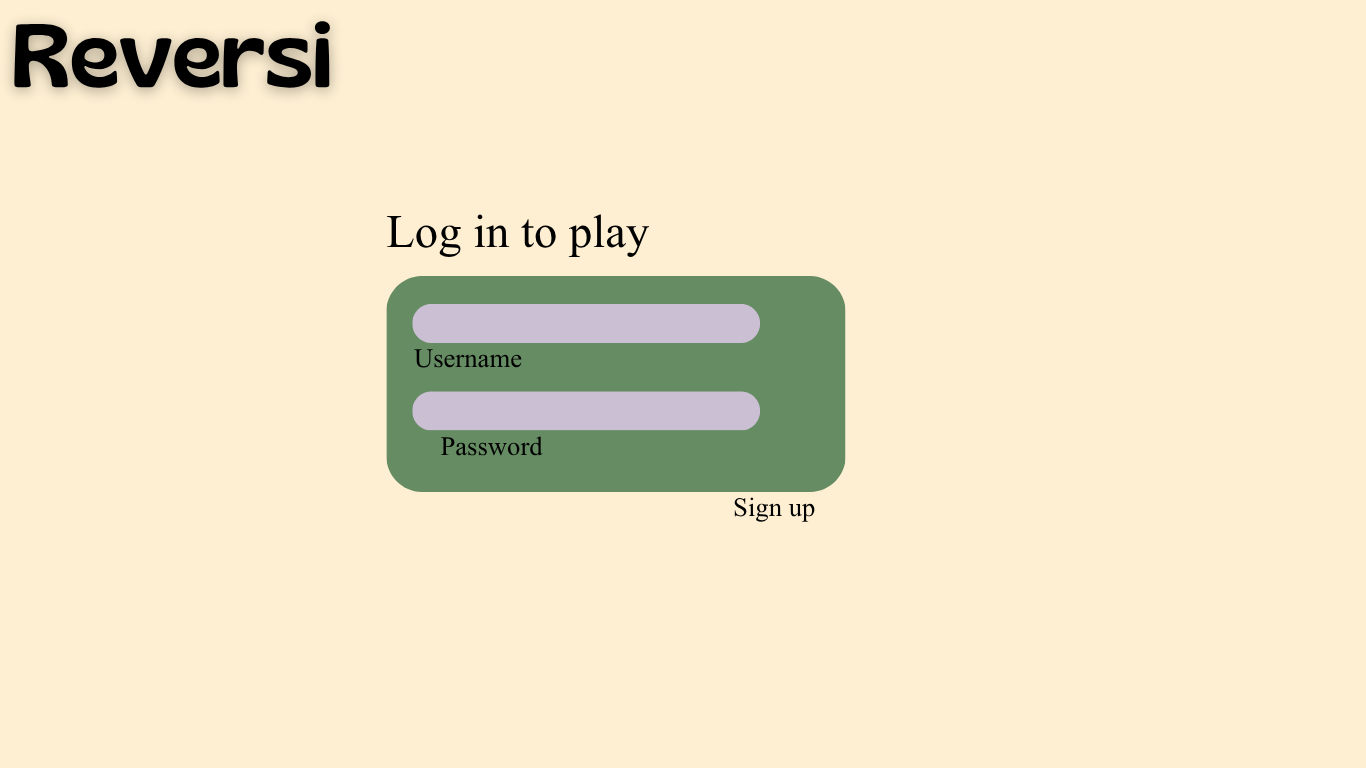
\includegraphics[width=\linewidth]{figures/ui_sign_in.png}\caption{Sign in (planned)}\end{subfigure}\hfill
\begin{subfigure}{0.48\textwidth}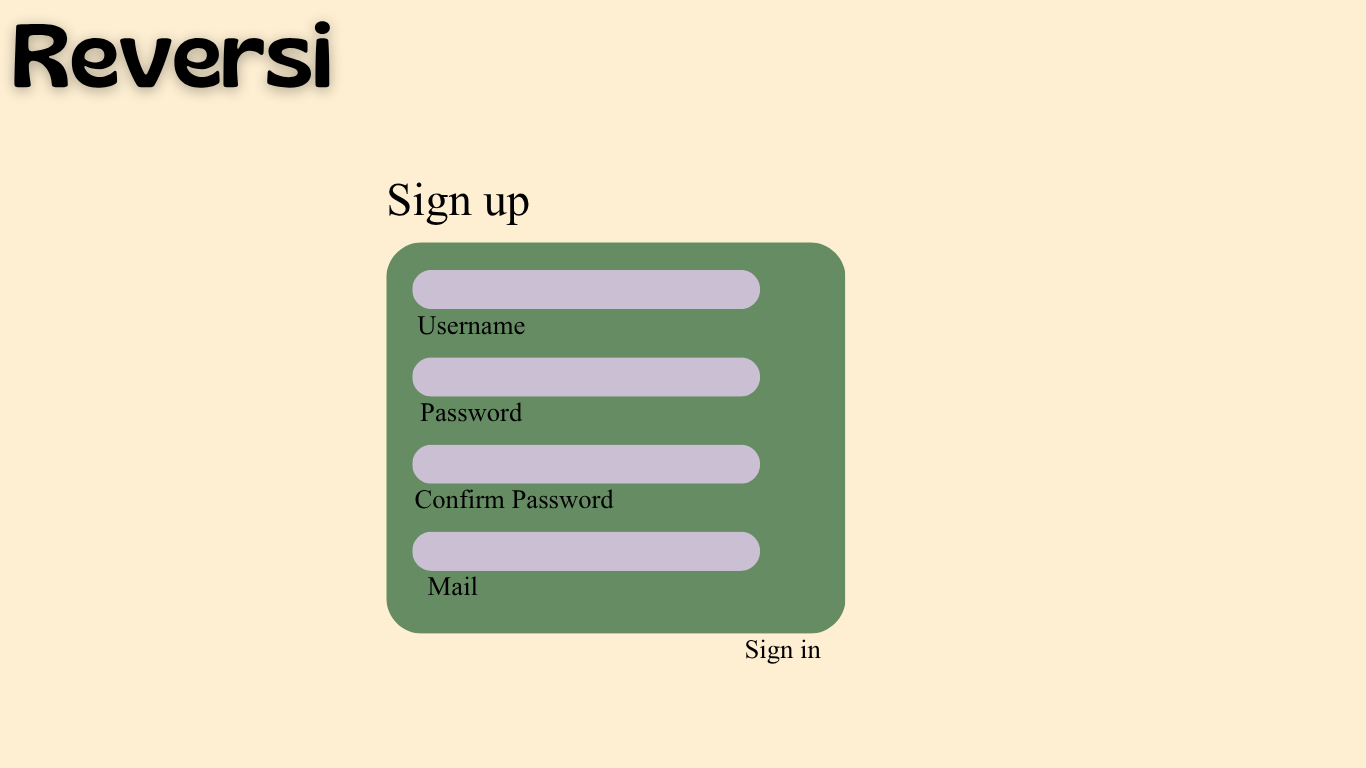
\includegraphics[width=\linewidth]{figures/ui_sign_up.png}\caption{Sign up (planned)}\end{subfigure}\\[6pt]
\begin{subfigure}{0.48\textwidth}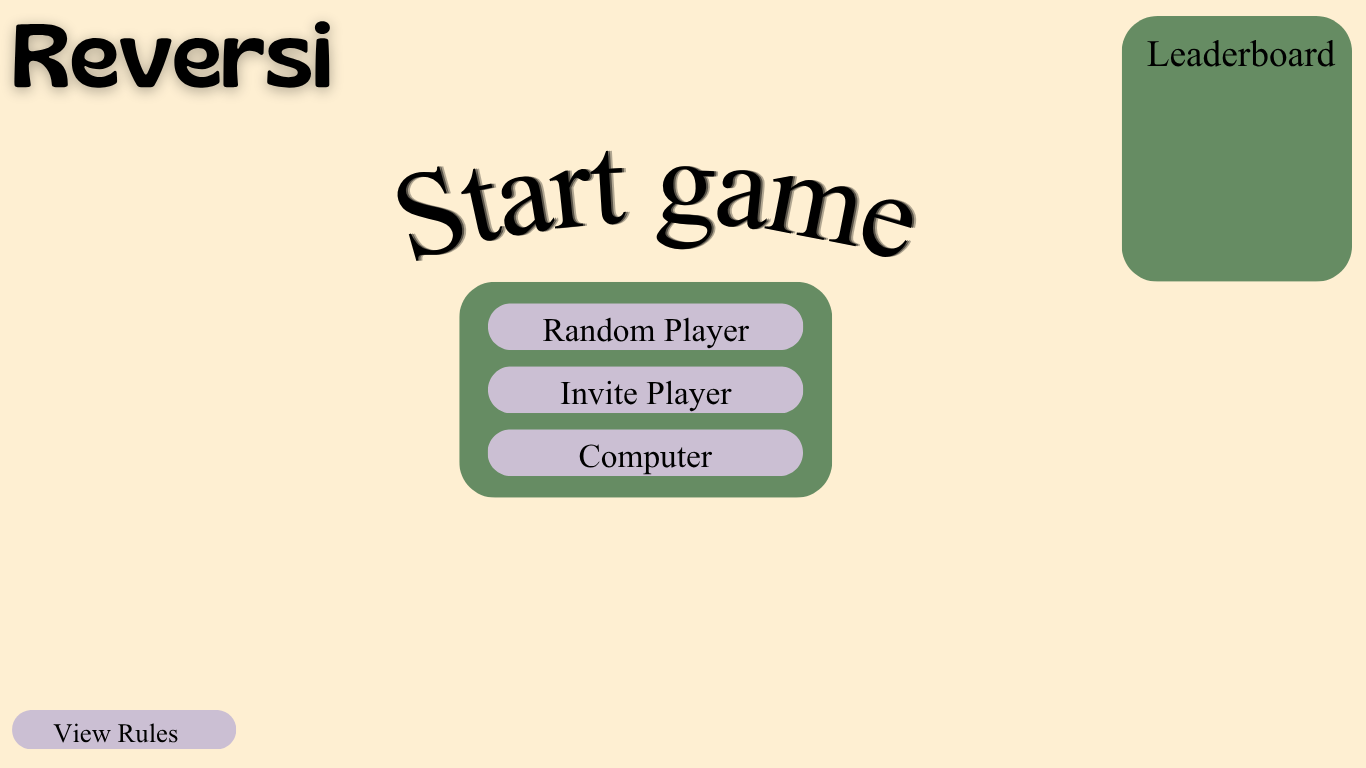
\includegraphics[width=\linewidth]{figures/ui_lobby.png}\caption{Lobby -- LobbyPage}\end{subfigure}\hfill
\begin{subfigure}{0.48\textwidth}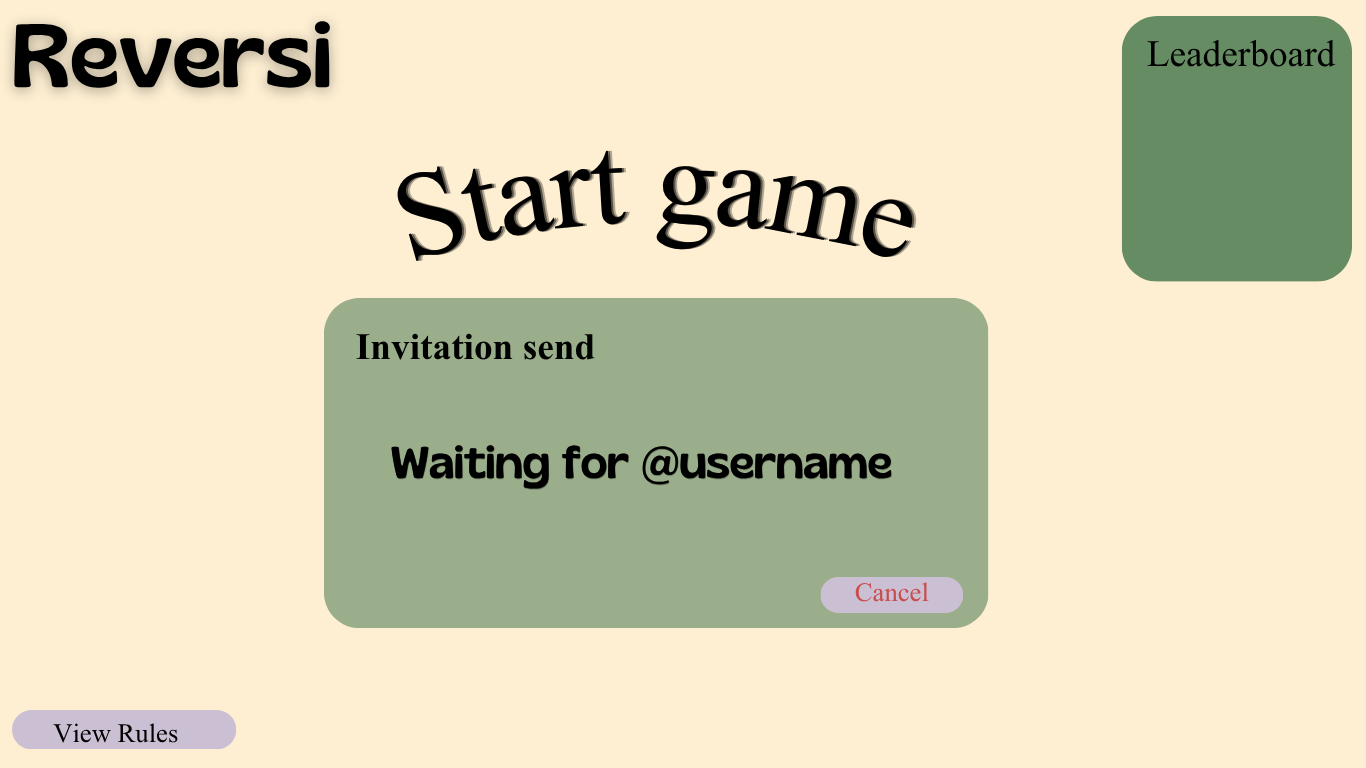
\includegraphics[width=\linewidth]{figures/ui_invite.png}\caption{Invite a player (planned)}\end{subfigure}\\[6pt]
\begin{subfigure}{0.48\textwidth}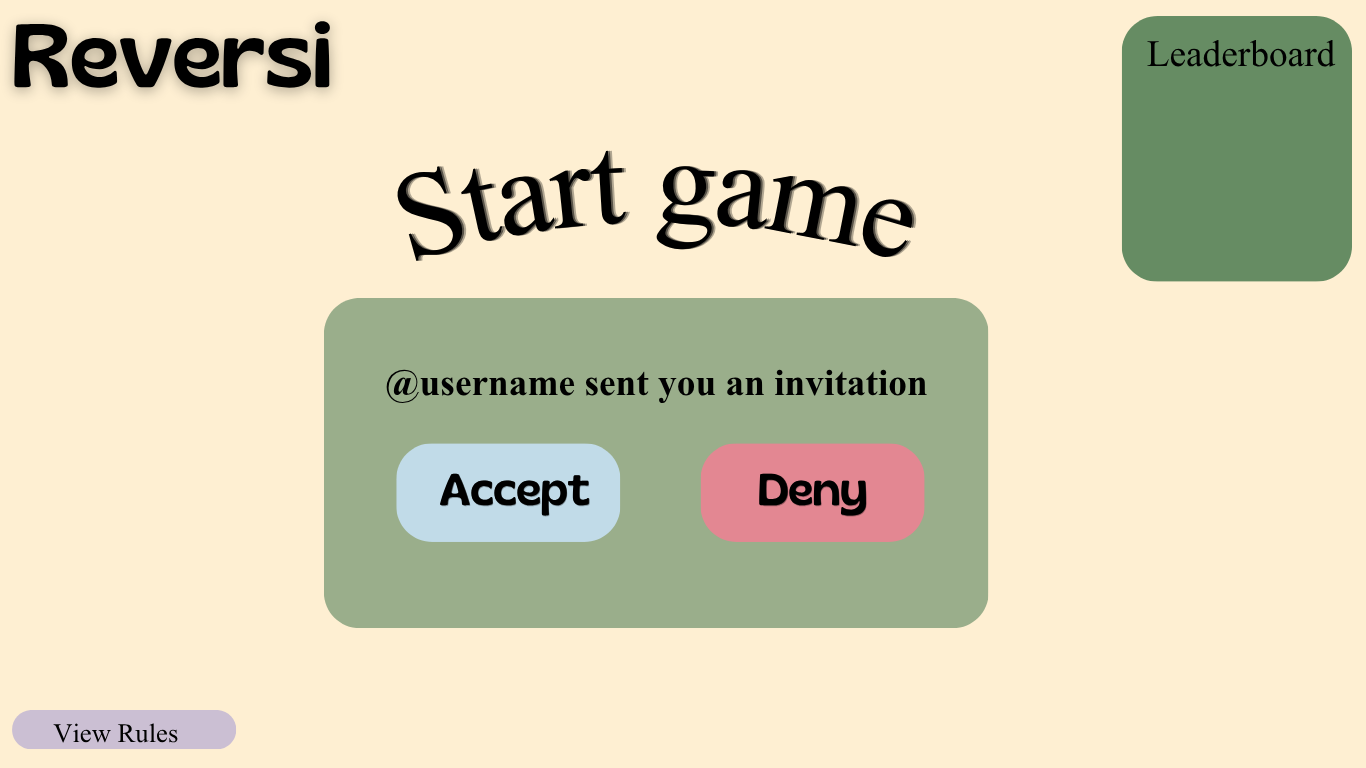
\includegraphics[width=\linewidth]{figures/ui_invitation_received.png}\caption{Invitation received (planned)}\end{subfigure}\hfill
\begin{subfigure}{0.48\textwidth}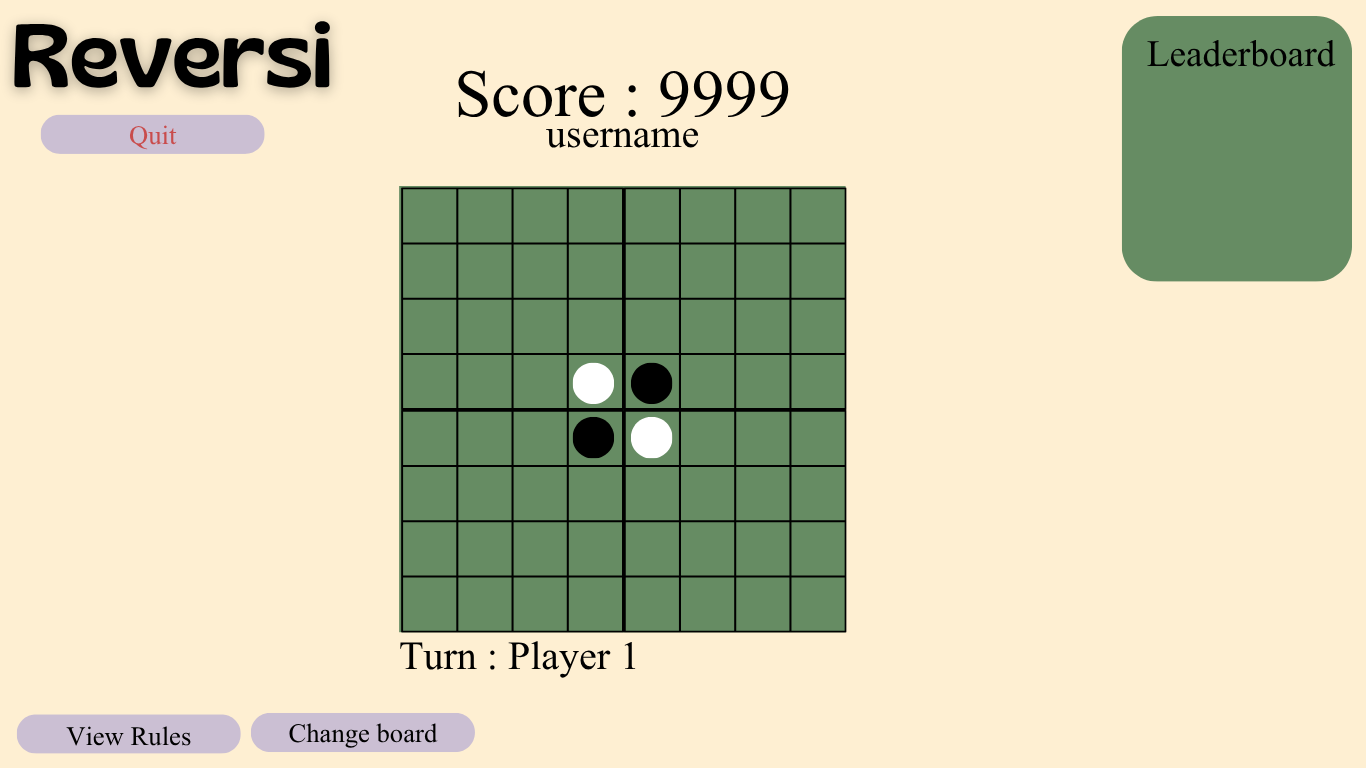
\includegraphics[width=\linewidth]{figures/ui_game.png}\caption{Game board -- GamePage}\end{subfigure}\\[6pt]
\begin{subfigure}{0.48\textwidth}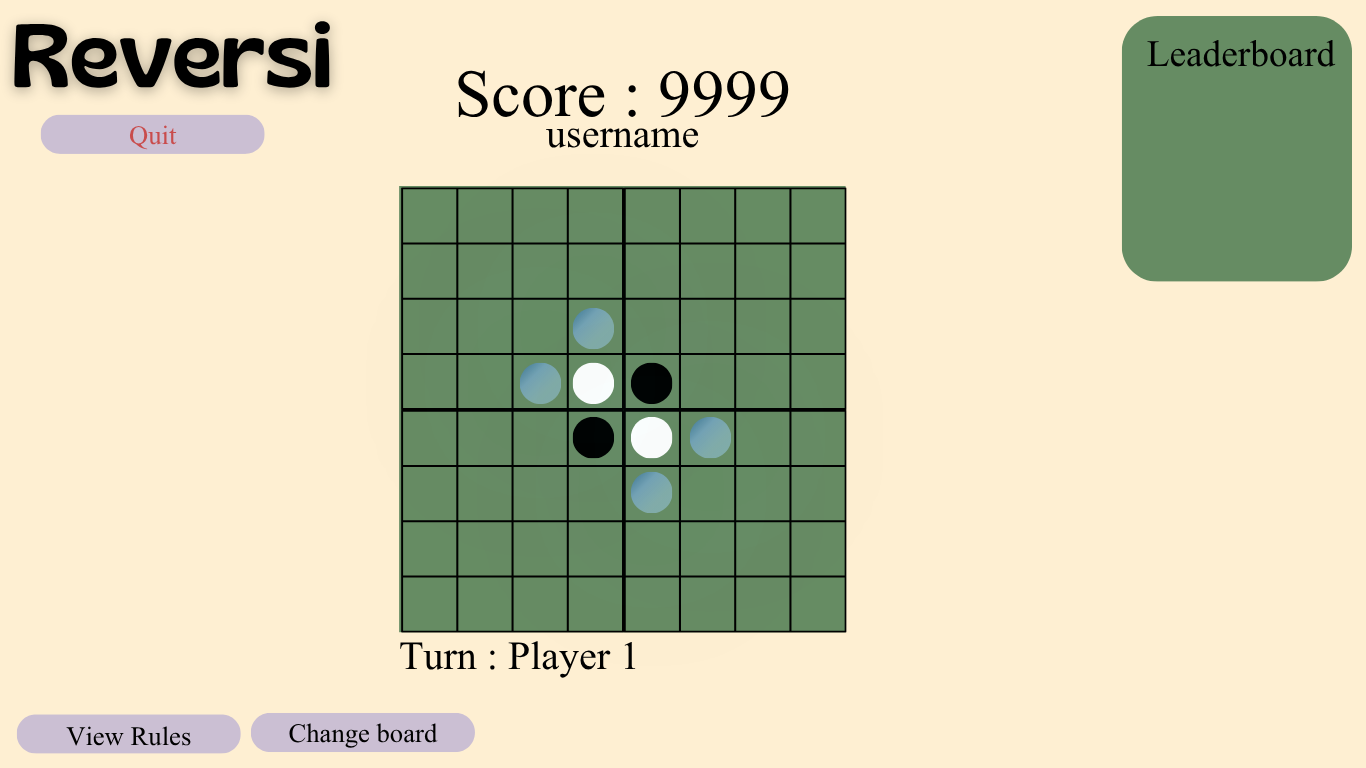
\includegraphics[width=\linewidth]{figures/ui_game_highlight.png}\caption{Legal moves highlighted (UC-02, variation 1$'$)}\end{subfigure}
\caption{User interface mock-ups}\label{fig:ui}
\end{figure}

\begin{tabularx}{\textwidth}{l L L}
\toprule
\textbf{Screen} & \textbf{Elements} & \textbf{Design classes / states}\\ \midrule
Lobby & Random player, invite player, computer; leaderboard; rules & LobbyPage.startGame(); SM-3 Lobby\\
Game board & Board, score, whose turn, quit, change board, leaderboard & GamePage.render(), play(), leave(); SM-4\\
Highlighted moves & Light-blue discs on legal squares & Board.getValidMoves(); UC-02 step 1\\
Sign in / up, invite & Account and invitation screens & Planned extension; SM-6 grey states\\
\bottomrule
\end{tabularx}

% ================================================================= 6 state machines
\section{State Machines}\label{sec:sm}

Following section 3.2.1 of the brief, the behaviour is shown as a hierarchy of state machines. The four required diagrams are two state diagrams and two sub-state diagrams; every transition is named and has a guard where a choice is made:

\begin{center}
\begin{tabular}{l l l}
\toprule
\textbf{Level} & \textbf{Server side (Game)} & \textbf{Client side (GamePage)}\\ \midrule
State diagram & SM-1 Game (GameStatus) & SM-3 GamePage\\
Sub-state diagram & SM-2 IN\_PROGRESS & SM-4 Playing\\ \midrule
Extra & SM-5 Cell & SM-6 Client navigation (target UI)\\
\bottomrule
\end{tabular}
\end{center}

State names match \texttt{GameStatus} (WAITING, IN\_PROGRESS, FINISHED) and the server status \texttt{cancelled}.

\fig[0.85\textwidth]{sm1_game.png}{SM-1: Game -- state diagram}
\fig[0.95\textwidth]{sm2_in_progress.png}{SM-2: Game IN\_PROGRESS -- sub-state diagram}
\fig[0.85\textwidth]{sm3_game_page.png}{SM-3: GamePage -- state diagram}
\fig[0.95\textwidth]{sm4_playing.png}{SM-4: GamePage Playing -- sub-state diagram}
\fig[0.7\textwidth]{sm5_cell.png}{SM-5: Cell -- state diagram (extra)}
\fig{sm6_client_navigation.png}{SM-6: Client navigation of the target UI (extra, matches the mock-ups)}

% ================================================================= 7 sequence diagrams
\section{Sequence Diagrams}\label{sec:sd}

The four sequence diagrams use UML 2.x frames (\texttt{sd}, \texttt{alt}, \texttt{opt}, \texttt{loop}, \texttt{break}, \texttt{ref}). There are two main diagrams, each with one sub-sequence diagram referenced by a \texttt{ref} fragment:

\begin{tabularx}{\textwidth}{l l L}
\toprule
\textbf{Diagram} & \textbf{Use case} & \textbf{Shows}\\ \midrule
SD-1 & UC-01 Join Game & Lobby to server, waiting loop with cancel (Ext 1a, 1b)\\
SD-1a & UC-01 step 2 & Pairing, random colours, building the starting board (Ext 2a)\\
SD-2 & UC-02 Make Move & Move from click to saved board; illegal move (Ext 2a)\\
SD-2a & UC-03 / UC-04 & Pass the turn, skip a turn, or end the game\\
\bottomrule
\end{tabularx}

Every message is a real operation from Figure~\ref{fig:domain_class_diagram.png} or Figure~\ref{fig:system_class_diagram.png}. Notes give the matching use case step or extension.

\fig{sd1_join_game.png}{SD-1: Join Game (UC-01)}
\fig[0.85\textwidth]{sd1a_pair_players.png}{SD-1a: Pair players and assign colours}
\fig{sd2_make_move.png}{SD-2: Make Move (UC-02)}
\fig[0.85\textwidth]{sd2a_turn_or_end.png}{SD-2a: Pass turn, skip turn or end game (UC-03, UC-04)}

% ================================================================= 8 communication diagrams
\section{Communication Diagrams}\label{sec:cd}

Each communication (collaboration) diagram is drawn from one sequence diagram, with the same objects and messages. Numbers show the nesting of calls (1.1 is called while handling 1), letters show alternative branches, \texttt{*} shows repetition, and guards are in square brackets.

\fig[0.7\textwidth]{cd1_join_game.png}{CD-1: Join Game (from SD-1)}
\fig[0.85\textwidth]{cd1a_pair_players.png}{CD-1a: Pair players and assign colours (from SD-1a)}
\fig[0.75\textwidth]{cd2_make_move.png}{CD-2: Make Move (from SD-2)}
\fig[0.85\textwidth]{cd2a_turn_or_end.png}{CD-2a: Pass turn, skip turn or end game (from SD-2a)}

% ================================================================= 9 class skeletons
\section{Class Skeletons}\label{sec:skeletons}

The skeletons come from the refined class diagrams and use our implementation languages: Python for the server and JavaScript for the browser. Each class shows its main attributes and methods with a short docstring; bodies are left empty. The full implementation is on GitHub.

\subsection{Game rules -- \texttt{domain.py}}
\lstinputlisting[language=Python]{../class_skeletons/domain.py}
\subsection{Server -- \texttt{server.py}}
\lstinputlisting[language=Python]{../class_skeletons/server.py}
\subsection{Browser client -- \texttt{client.js}}
\lstinputlisting[language=JavaScript]{../class_skeletons/client.js}

% ================================================================= 10 vulnerability review
\section{Technical Vulnerability Review}\label{sec:vuln}

The Phase 1 feedback asked for a formal review of technical vulnerabilities. We used the STRIDE headings (Spoofing, Tampering, Repudiation, Information disclosure, Denial of service, Elevation of privilege) and checked each risk against the classes of Figures~\ref{fig:domain_class_diagram.png} and~\ref{fig:system_class_diagram.png}.

\small
\begin{longtable}{>{\raggedright\arraybackslash}p{0.6cm} >{\raggedright\arraybackslash}p{2.0cm} >{\raggedright\arraybackslash}p{2.8cm} >{\raggedright\arraybackslash}p{4.0cm} >{\raggedright\arraybackslash}p{3.1cm} >{\raggedright\arraybackslash}p{1.6cm}}
\toprule
\textbf{\#} & \textbf{Threat} & \textbf{Example attack} & \textbf{Mitigation} & \textbf{Class / operation} & \textbf{Status}\\ \midrule\endhead
V1 & Spoofing & Player B sends a move as Player A & Each seat has a random secret token, returned only to that browser and checked on every action with a constant-time compare & GameRecord.colorForToken, GameService.makeMove & Mitigated\\
V2 & Tampering & Client sends a fake board or an illegal square & The server is the only authority. The client sends only (row, col); placePiece re-checks the rules and raises InvalidMoveError & Board.placePiece, Game.playTurn & Mitigated\\
V3 & Tampering & Playing out of turn or after the end & NotYourTurnError, GameOverError & Game.playTurn & Mitigated\\
V4 & Tampering (race) & Two moves for the same game at the same moment & Each action runs in one database transaction with a row lock; move numbers are unique per game & GameService, MoveRecord & Mitigated\\
V5 & Tampering (bad input) & Non-numeric row, board size 7, 1000-character name & Numbers checked, Board.inBounds, size must be 6/8/10, name 1--30 characters & GameService, Board & Mitigated\\
V6 & Information disclosure / XSS & Name like \texttt{<script>} shown to the opponent & Names are inserted as text (textContent / escapeHtml), never as HTML & ApiClient.escapeHtml, GamePage.render & Mitigated\\
V7 & Information disclosure & Token stolen from the browser & Token stored for that game only and useless once it ends; V6 also protects it & ApiClient.saveSeat & Accepted\\
V8 & Information disclosure & Token sniffed on the network & Must be served over HTTPS when deployed & Deployment (Fig.~\ref{fig:deployment_diagram.png}) & Open (deploy)\\
V9 & Spoofing & Playing under someone else's name to change their leaderboard & No accounts in this version; a name is not proof of identity. Sign-in is a planned extension (mock-ups) & PlayerProfile & Accepted\\
V10 & Denial of service & Opponent stops responding so the game never ends & 30\,s reconnection window, then forfeit; stale lobby games are cancelled & GameService.pollGame, joinOnlineGame & Mitigated\\
V11 & Denial of service & Making the computer think forever & Search depth is fixed (3, or 2 on 10$\times$10); the computer only moves when asked by the seated player & ComputerPlayer & Mitigated\\
V12 & Denial of service & Flooding the API with requests & History limited to 50 rows and leaderboard to 20; no rate limiting yet & GameAPI & Open\\
V13 & Elevation of privilege & Debug pages or a known secret key in production & Secret key, debug flag and allowed hosts set by environment variables & settings.py & Open (deploy)\\
V14 & Repudiation & ``I never played that move'' & Every move is stored with number, colour, square and time & MoveRecord & Mitigated\\
V15 & CSRF & Another site makes the browser send a move & No cookies or sessions; the token must be sent in a custom header that other sites cannot add & GameAPI, ApiClient.api & Mitigated\\
\bottomrule
\end{longtable}
\normalsize

% ================================================================= 11 consistency review
\section{Design Consistency Review}\label{sec:review}

Before submission we did a structured walkthrough of all Phase 2 diagrams against the refined class diagrams, which are the reference for names. Table~\ref{tab:review} lists what we found and how it was fixed in this document. The original working files are kept on GitHub for traceability.

\small
\begin{longtable}{>{\raggedright\arraybackslash}p{2.6cm} >{\raggedright\arraybackslash}p{6.0cm} >{\raggedright\arraybackslash}p{6.4cm}}
\caption{Inconsistencies found and fixed}\label{tab:review}\\
\toprule
\textbf{Item} & \textbf{Problem found} & \textbf{Fix}\\ \midrule\endhead
Sequence diagrams SD-1, SD-1a & Used classes that are not in the design (LobbyController, Matchmaker) and operations such as startGame(), placeStartingDiscs(), assignColours() & Redrawn with LobbyPage, ApiClient, GameAPI, GameService, GameRecord, Game, Board and their real operations (joinOnlineGame, buildGame, initialize, start). Same fragments kept.\\
Sequence diagrams SD-2, SD-2a & Planned in the work split but not yet drawn & Drawn for UC-02 and UC-03/UC-04 so that there are four sequence diagrams.\\
Communication diagrams & Used classes not in the design (ScoreManager, Database) and operations surrender(), validate(), declareWinner(); numbering did not match the sequence diagrams; one label was in French (``Coup invalide''); one file ended with \texttt{@endum} & Redrawn from SD-1, SD-1a, SD-2 and SD-2a with the same objects and messages, as the brief asks. Illegal-move and end-of-game cases are kept as guarded branches.\\
Object diagrams & Attribute names differed from the class diagram (currentTurnIndex, GameState, isObstacle); the computer was Black although UC-05 says the player is Black; cell E5 had col = 4; ``IA'' instead of AI; scores at the start were 0 & Redrawn: currentPlayerIndex, GameStatus, no obstacles, human player is Black, correct 0-based coordinates, starting score 2 each. The mid-game diagram now shows a consistent move number (38 moves for 42 pieces).\\
State machines & Two sets existed. The first draft had Paused and AwaitingReconnection states, but pause was dropped from the design. The navigation diagram had spelling mistakes and unnamed transitions & The four required diagrams use GameStatus names; every transition is named, with guards. Reconnection is a 30\,s guard instead of a state. Cell and navigation diagrams kept as extras, with spelling fixed and all transitions named.\\
Use cases & Difficulty levels written as easy/medium/hard; online pairing also filtered by difficulty; two variations numbered 1$'$ & Easy/normal/hard everywhere; online pairing only uses board size (difficulty only applies to computer games); variations renumbered.\\
Mock-ups vs.\ design & Sign-in, sign-up and invite screens have no matching classes & Marked as planned extensions in Section~\ref{sec:ui}, UC-01 variation 1$''$, SM-6 and V9.\\
Meeting records & Meeting of 14/10 gave the next meeting as 28/10, but the team met on 21/10 & Corrected in Section~\ref{sec:minutes}.\\
\bottomrule
\end{longtable}
\normalsize

% ================================================================= 12 minutes
\section{Team Meeting Records}\label{sec:minutes}

The team works in short Agile iterations: a weekly meeting (Wednesday, 12:00) to review progress and assign tasks, with the shared Google Doc and GitHub used between meetings.

\subsection{Meeting 1 -- Wednesday 7 October 2026, 12:00}
\begin{tabularx}{\textwidth}{>{\bfseries}p{3cm} L}
Attendance & Anna, Ailbhe, Tim, Michel (Blanche and Diane absent)\\
Agenda & Assign the Phase 2 tasks; front end and back end of the game\\
Discussion & How to split the game between the browser client and the server\\
Decisions & Python/Django backend with an HTML/JavaScript client. The backend skeleton was merged on GitHub during the meeting (pull request \#2).\\
Actions & Object diagrams and communication diagrams -- Blanche\newline
Revised use cases and sequence diagrams -- Tim\newline
Sequence diagrams -- Ailbhe\newline
Refined class diagrams and class skeletons -- Michel\newline
State machine diagrams and walkthrough -- Anna\newline
UI mock-ups, state machine and meeting notes -- Diane\\
Next meeting & 14 October 2026, 12:00\\
\end{tabularx}

\subsection{Meeting 2 -- Wednesday 14 October 2026, 12:00}
\begin{tabularx}{\textwidth}{>{\bfseries}p{3cm} L}
Attendance & Tim, Michel, Anna, Ailbhe, Blanche, Diane (all)\\
Agenda & Share and discuss individual work so far\\
Discussion & Progress on each person's part; first UI mock-ups (12/10)\\
Decisions & Keep the same work split until the deadline\\
Actions & Same owners as Meeting 1\\
Next meeting & 21 October 2026, 12:00\\
\end{tabularx}

\subsection{Meeting 3 -- Wednesday 21 October 2026, 12:00}
\begin{tabularx}{\textwidth}{>{\bfseries}p{3cm} L}
Attendance & Diane, Blanche, Tim, Michel (Anna and Ailbhe absent)\\
Agenda & What is left for deliverable 2\\
Discussion & State machine and sequence diagrams; what went wrong in Phase 1 and how to improve (lecturer feedback)\\
Decisions & Add the technical vulnerability review asked for in the feedback; put all diagram sources on GitHub (\texttt{docs/phase2/})\\
Actions & Vulnerability review -- Michel\newline Review the scenarios -- Ailbhe\\
Next meeting & 28 October 2026, 12:00\\
\end{tabularx}

\subsection{Task board (status on 22 October 2026)}
\small
\begin{tabularx}{\textwidth}{L l l l}
\toprule
\textbf{Task} & \textbf{Owner} & \textbf{Status} & \textbf{Date}\\ \midrule
Revised use cases and use case diagram & Tim & Done & 22/10\\
Sequence diagrams SD-1, SD-1a & Tim & Done & 22/10\\
Sequence diagrams SD-2, SD-2a & Michel (integration) & Done & 22/10\\
Object diagrams & Blanche & Done & 21/10\\
Communication diagrams & Blanche & Done & 21/10\\
Refined class diagrams & Michel & Done & 20/10\\
Class skeletons & Michel & Done & 20/10\\
Technical vulnerability review & Michel & Done & 20/10\\
State machine diagrams & Anna & Done & 21/10\\
Client navigation state machine & Diane & Done & 21/10\\
UI mock-ups & Diane & Done & 12/10\\
Meeting notes & Diane & Done & 21/10\\
Design consistency review and final report & Michel & Done & 22/10\\
Provisional source code (next phase) & All & In progress & 13/11\\
\bottomrule
\end{tabularx}
\normalsize

\subsection{Activity log (from GitHub commits and Google Doc history)}
\small
\begin{tabularx}{\textwidth}{l l L}
\toprule
\textbf{Date} & \textbf{Who} & \textbf{Activity}\\ \midrule
Mon 05/10 & Ailbhe & Doc: edits to the shared document\\
Mon 05/10 & Anna & GitHub: project structure added\\
Wed 07/10 & Michel, Anna & GitHub: Django backend started; pull request \#2 reviewed and merged by Anna; game logic moved into the backend\\
Wed 07/10 & Blanche & Doc: edits to the shared document\\
Wed 07/10 & Michel & GitHub: first playable version (game rules, API, client)\\
Mon 12/10 & Diane & Doc: UI mock-ups\\
Tue 20/10 & Michel & Doc and GitHub: refined class diagrams, class skeletons, vulnerability review\\
Tue 20/10 & Anna & Doc: edits to the shared document\\
Wed 21/10 & Blanche & GitHub and Doc: object diagrams, communication diagrams\\
Wed 21/10 & Diane & GitHub: navigation state machine; Doc: meeting notes\\
Wed 21/10 & Anna & Doc: edits to the shared document\\
Thu 22/10 & Tim & Doc: use cases and sequence diagrams tab\\
Thu 22/10 & Michel & GitHub: Phase 2 branches merged into \texttt{main}; consistency review; final report\\
\bottomrule
\end{tabularx}
\normalsize

% ================================================================= 13 AI
\section{Use of AI}\label{sec:ai}

This declaration follows the module's guidance on AI tools and DCU's academic integrity policy. A generative AI assistant was used in Phase 2 as a support tool only. It did not replace the team's analysis or design work.

\textbf{Where AI was used}
\begin{itemize}
  \item \textbf{Formatting the report.} Typesetting this document in \LaTeX, laying out tables and figures, and putting all diagrams into one notation (PlantUML) so that they look the same.
  \item \textbf{Checking consistency.} Cross-checking class and operation names between the team's diagrams and the refined class diagrams. The team reviewed each issue found and decided how to fix it (Section~\ref{sec:review}).
  \item \textbf{Help when the team was blocked.} Fixing PlantUML syntax errors, explaining UML 2.x notation (sequence diagram fragments, communication diagram numbering) and the STRIDE headings. In a few places the team was stuck and used the assistant for a starting draft: the PlantUML layout of the refined class diagrams (from our own Phase 1 diagram and code), the class skeletons, and the sequence diagrams SD-2 and SD-2a. Each draft was then checked line by line against our use cases and code and corrected by team members.
\end{itemize}

\textbf{What came from the team.} The requirements, use cases, game features, client/server split, class structure and relationships, state machine states and transitions, the mock-ups and every design decision (random colours, no pause, no rematch, 30\,s forfeit, difficulty levels) come from the team's own analysis and meetings. No AI output was copied in without review.

\textbf{Accountability.} The team has read and checked every diagram, table and line of code in this report, takes full responsibility for it, and can explain any part of it.

% ================================================================= appendix
\appendix
\section{Diagram Source Files}\label{app:sources}

All diagrams in this report were drawn with PlantUML. The text files are in the repository folder\\ \texttt{docs/phase2/report/diagrams/} and can be rendered with:

\texttt{java -jar plantuml.jar -tpng -o ../figures *.puml}

The team's working files (Mermaid object and state diagrams, first communication diagrams) are kept in \texttt{docs/phase2/} and in the root of the repository.

\scriptsize
\newcommand{\src}[1]{\subsection*{\normalsize\texttt{\detokenize{#1}}}\lstinputlisting[language=PlantUML]{diagrams/#1}}
\src{style.iuml}
\src{use_case_diagram.puml}
\src{domain_class_diagram.puml}
\src{system_class_diagram.puml}
\src{deployment_diagram.puml}
\src{od1_computer_game_start.puml}
\src{od2_online_game_midway.puml}
\src{sm1_game.puml}
\src{sm2_in_progress.puml}
\src{sm3_game_page.puml}
\src{sm4_playing.puml}
\src{sm5_cell.puml}
\src{sm6_client_navigation.puml}
\src{sd1_join_game.puml}
\src{sd1a_pair_players.puml}
\src{sd2_make_move.puml}
\src{sd2a_turn_or_end.puml}
\src{cd1_join_game.puml}
\src{cd1a_pair_players.puml}
\src{cd2_make_move.puml}
\src{cd2a_turn_or_end.puml}

\end{document}
